\section{Introduction}
\label{sec:introduction}

Smart Power Grid~\cite{huang11} is a prime example of Cyber-Physical System 
(CPS) where the goal is to have embedded computing devices monitor and control 
distributed generation, storage and transfer of power in a safe, reliable, 
efficient and secure manner. Ensuring stability and correctness (both logical and temporal)
of the system as a whole is a major challenge in CPS design. Any incorrectness or 
instability in one component can impact the same features of other components. 
For example, an action in the physical domain could affect the network domain and 
vice-versa, thus making correct scheduling of these actions paramount to overall system
stability. The fundamental challenge in developing a design framework that
unifies the various components is the heterogeneity of the component types,
resulting in semantic gaps that must be bridged. 

% comparison
Existing papers largely consider the stability of one or two components in
isolation. For example, network delays affect system stability and considerable
work focusses on determining system stability bounds as a function of injected
delay~\cite{hespanha07}. Results from switched-systems theory~\cite{donkers11}
model the stability of the plant. Hybrid automata~\cite{henzinger96} and timed
I/O automata~\cite{alur94} represent a simultaneous mix of continuous and
discrete states in the verification process~\cite{chutinan03,tomlin03}.
Real-time scheduling is traditionally a function of \emph{a priori} time
bounds~\cite{liu00}. To consider components individually, or in pairs, requires
that they be very stable such that the composition of the components into a CPS
is stable.

In our work, we employ a fundamentally different approach that composes
correctness instead of functionality. The basic idea, depicted in
Figure~\ref{fig:invariant_conjunction}, is to express the stability and
correctness constraints of all components in the form of logical {\em invariants} 
and ensure that system actions are performed only if and when they are guaranteed not 
to violate the conjunction of these invariants. This approach is not only limited
to smart power grid design but can also be generalized to different cyber-physical systems 
with different functionalities. 

\begin{figure}[htb]
  \begin{center}
%    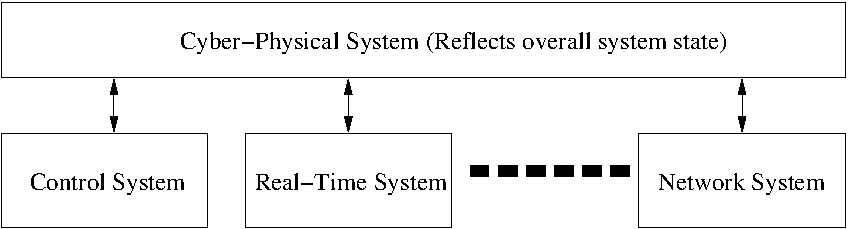
\includegraphics[width=0.45\textwidth]{Figures/cps-n-domains.pdf}
     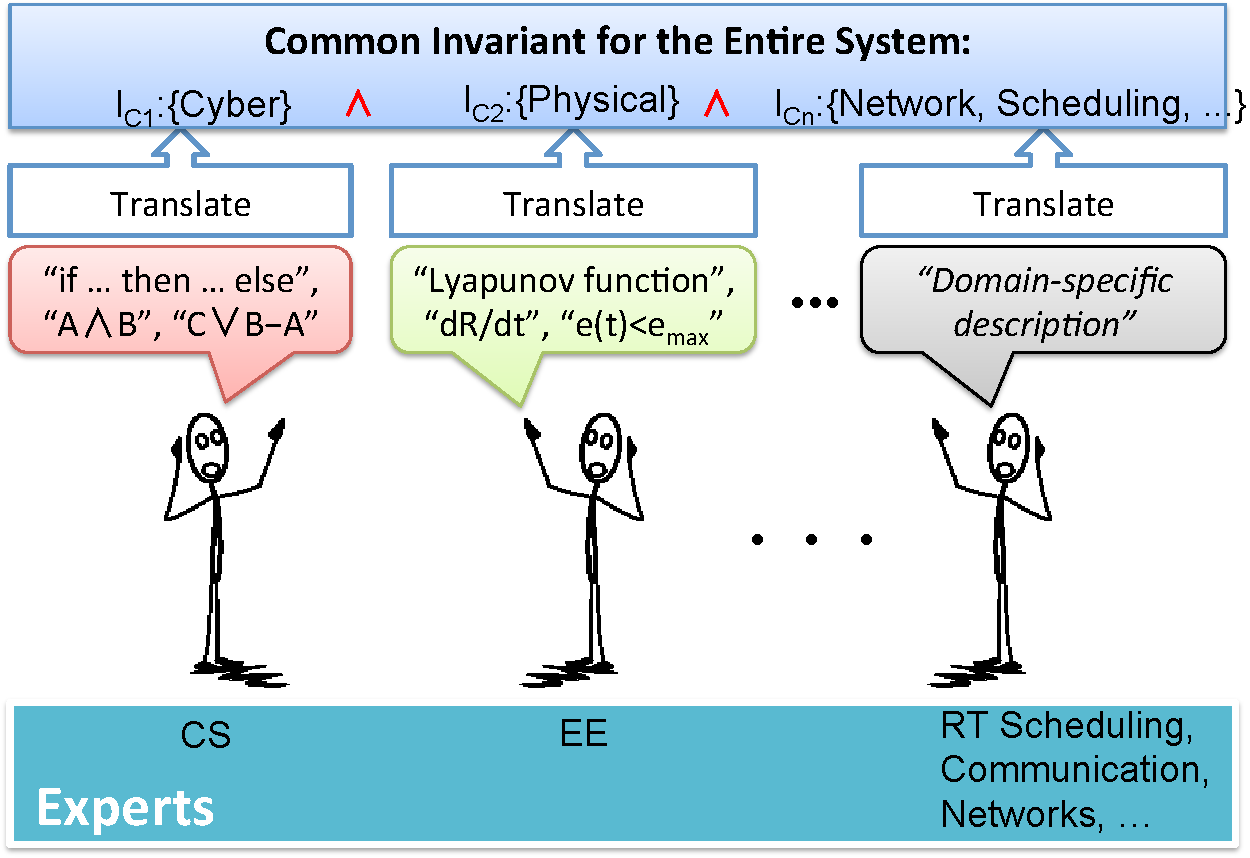
\includegraphics[width=0.9\columnwidth]{Figures/Invariant_Overview.pdf}
  \caption{Overview of invariant-based approach}
  \label{fig:invariant_conjunction}
  \end{center}
\end{figure}

The state of the physical system and, hence, its stability, is dependent on
power transfers (series of power migrations) initiated by the cyber algorithm
within each node in the system and by the state of the communication network
that carries messages between the cyber nodes to signal initiation and
acknowledgement of physical power migrations. The state and stability of the
communication network is in turn affected by the number of migration messages in
transit at any given time. In recent work[*****cite COMPSAC], we developed a 
scheduling invariant for our distributed, adaptive algorithm for scheduling power 
migrations between nodes in a smart grid and demonstrate that conjunction of such a
scheduling invariant and an invariant for physical system state is necessary to 
maintain overall system stability. In contrast to traditional real-time scheduling, 
{\em correct} scheduling in our context refers to initiating actions at appropriate 
times in a way that system stability is maintained rather than insisting that every 
action is initiated at a pre-defined time and must adhere to a pre-defined deadline. 
In order to improve efficiency along with stability, components in CPS must have 
certain amount of inter-component information. In the current paper, we focus on 
improving the efficiency while also maintaining the stability of smart grid nodes 
by exploiting the network congestion information obtained from Early Congestion 
Notification (ECN) scheme, wherein packets are marked indicating impending congestion,
instead of dropping them\cite{floyd1994tcp, ramakrishnan1999proposal, 
ramakrishnan2001addition}. We allow the smart grid nodes to sense the possible 
upcoming network congestion and change the amount of power being transferred with 
every power migrate message in order to compensate for reduced rate of power transfers.
As of our knowledge, this is the first work that explore ECN scheme from CPS context
for the benefit of physical system efficiency as well as take necessary action to 
reduce network congestion.

The rest of this paper is organized as follows. Section \ref{sec:related_work}
provides some background information and discusses related work. We present our
system model and assumptions in Section \ref{sec:assumptions}. Section
\ref{sec:phy_sched_analysis_and_invariants} presents our physical system 
invariant and adaptive scheduling invariant. Section \ref{sec:power_management_algo} 
presents our resulting power management algorithm. Our simulation setup is introduced 
in Section \ref{sec:simulation_setup} and results are presented in Section
\ref{sec:results}. Section \ref{sec:discussion} presents a brief discussion and
conclusions are presented in Section \ref{sec:conclusions}.

